\documentclass[12pt,a4paper]{article}

\usepackage{arxiv}

\usepackage{amsmath}
\usepackage{amsthm}
\usepackage{amssymb}

\usepackage[T1]{fontenc}    % use 8-bit T1 fonts
\usepackage[utf8]{inputenc} % allow utf-8 input

\usepackage{hyperref}        % hyperlinks
\usepackage{url}            % simple URL typesetting
\usepackage{booktabs}       % professional-quality tables
\usepackage{amsfonts}       % blackboard math symbols
\usepackage{nicefrac}       % compact symbols for 1/2, etc.
\usepackage{microtype}      % microtypography
\usepackage{cleveref}       % smart cross-referencing
\usepackage{graphicx}
\usepackage{natbib}
\usepackage{doi}

\usepackage{float}
\usepackage{caption}
\usepackage{subcaption}

\usepackage{multirow}

\DeclareMathOperator{\rank}{rank}
\makeatletter
\newenvironment{sqcases}{%
	\matrix@check\sqcases\env@sqcases
}{%
	\endarray\right.%
}
\def\env@sqcases{%
	\let\@ifnextchar\new@ifnextchar
	\left\lbrack
	\def\arraystretch{1.2}%
	\array{@{}l@{\quad}l@{}}%
}
\makeatother

\usepackage{hyperref}

\hypersetup{
	colorlinks=false, 
	urlcolor=blue,
	linkcolor=blue,
	citecolor=green,
	linkbordercolor={0 0 1}
}


\title{
	Filtering Input Data Errors in Model Error Calculations: Impact of Measurement Uncertainty on Mean Absolute Error Estimation\\
	\vspace{5mm}
	\textit{\large DRAFT VERSION}
} 

\date{Last update: \today}

\author{
	\vspace{5mm}Vasilii Piiadov\\
	\texttt{piyadov@alumni.usp.br} \\
}

\theoremstyle{definition}
\newtheorem{definition}{Definition}

\begin{document}
\maketitle
\begin{abstract}
This paper examines the impact of measurement uncertainty on Mean Absolute Error (MAE) calculations in statistical analysis and model validation. We derive analytical expressions for the distribution of absolute differences between observations under various uncertainty models, including delta function distributions for data without uncertainty and normal distributions for measurement errors. Our analysis demonstrates that conventional MAE calculations can lead to systematic overestimation when input data contains uncertainty, particularly in cases where the signal-to-noise ratio is low. We establish sufficient conditions under which standard MAE calculations remain approximately valid and propose methods for accurate MAE estimation in the presence of measurement uncertainty. The findings have significant implications for model validation in industrial applications where measurement precision affects performance assessment.

\end{abstract}

\section{Introduction}

Consider two sets of unknown true values $\{a_k\}$ and $\{b_k\}$ that are estimated through observations $\{x_k\}$ and $\{y_k\}$, respectively. The Mean Absolute Error (MAE) between the true values is defined as:

\begin{equation}
	h = \frac{1}{n} \sum\limits_{k=1}^{n} \left\vert a_k - b_k \right\vert
	\label{eq:gen_mae}
\end{equation}

In practical applications, we seek to calculate the MAE using the available dataset of observations $\{x_k\}$ and $\{y_k\}$. However, the relationship between observed and true MAE depends critically on the uncertainty characteristics of the measurement process.


\section{Distribution of absolute difference between observations}

Let $x \in X$ and $y \in Y$ represent single estimations of $a$ and $b$, respectively, modeled as random variables. We denote $F_X(x)$ and $F_Y(y)$ as the distribution functions describing the uncertainty in single observations, with corresponding probability density functions $f_X(x)$ and $f_Y(y)$. Note that these distribution functions depend on the true values $a$ and $b$ such that $x$ and $y$ serve as their estimators.

We consider the absolute difference $z$ between $x$ and $y$: $z \in Z$, where $Z = \left| X - Y \right|$ and $z \geq 0$.


\begin{figure}[H]
	\centering
	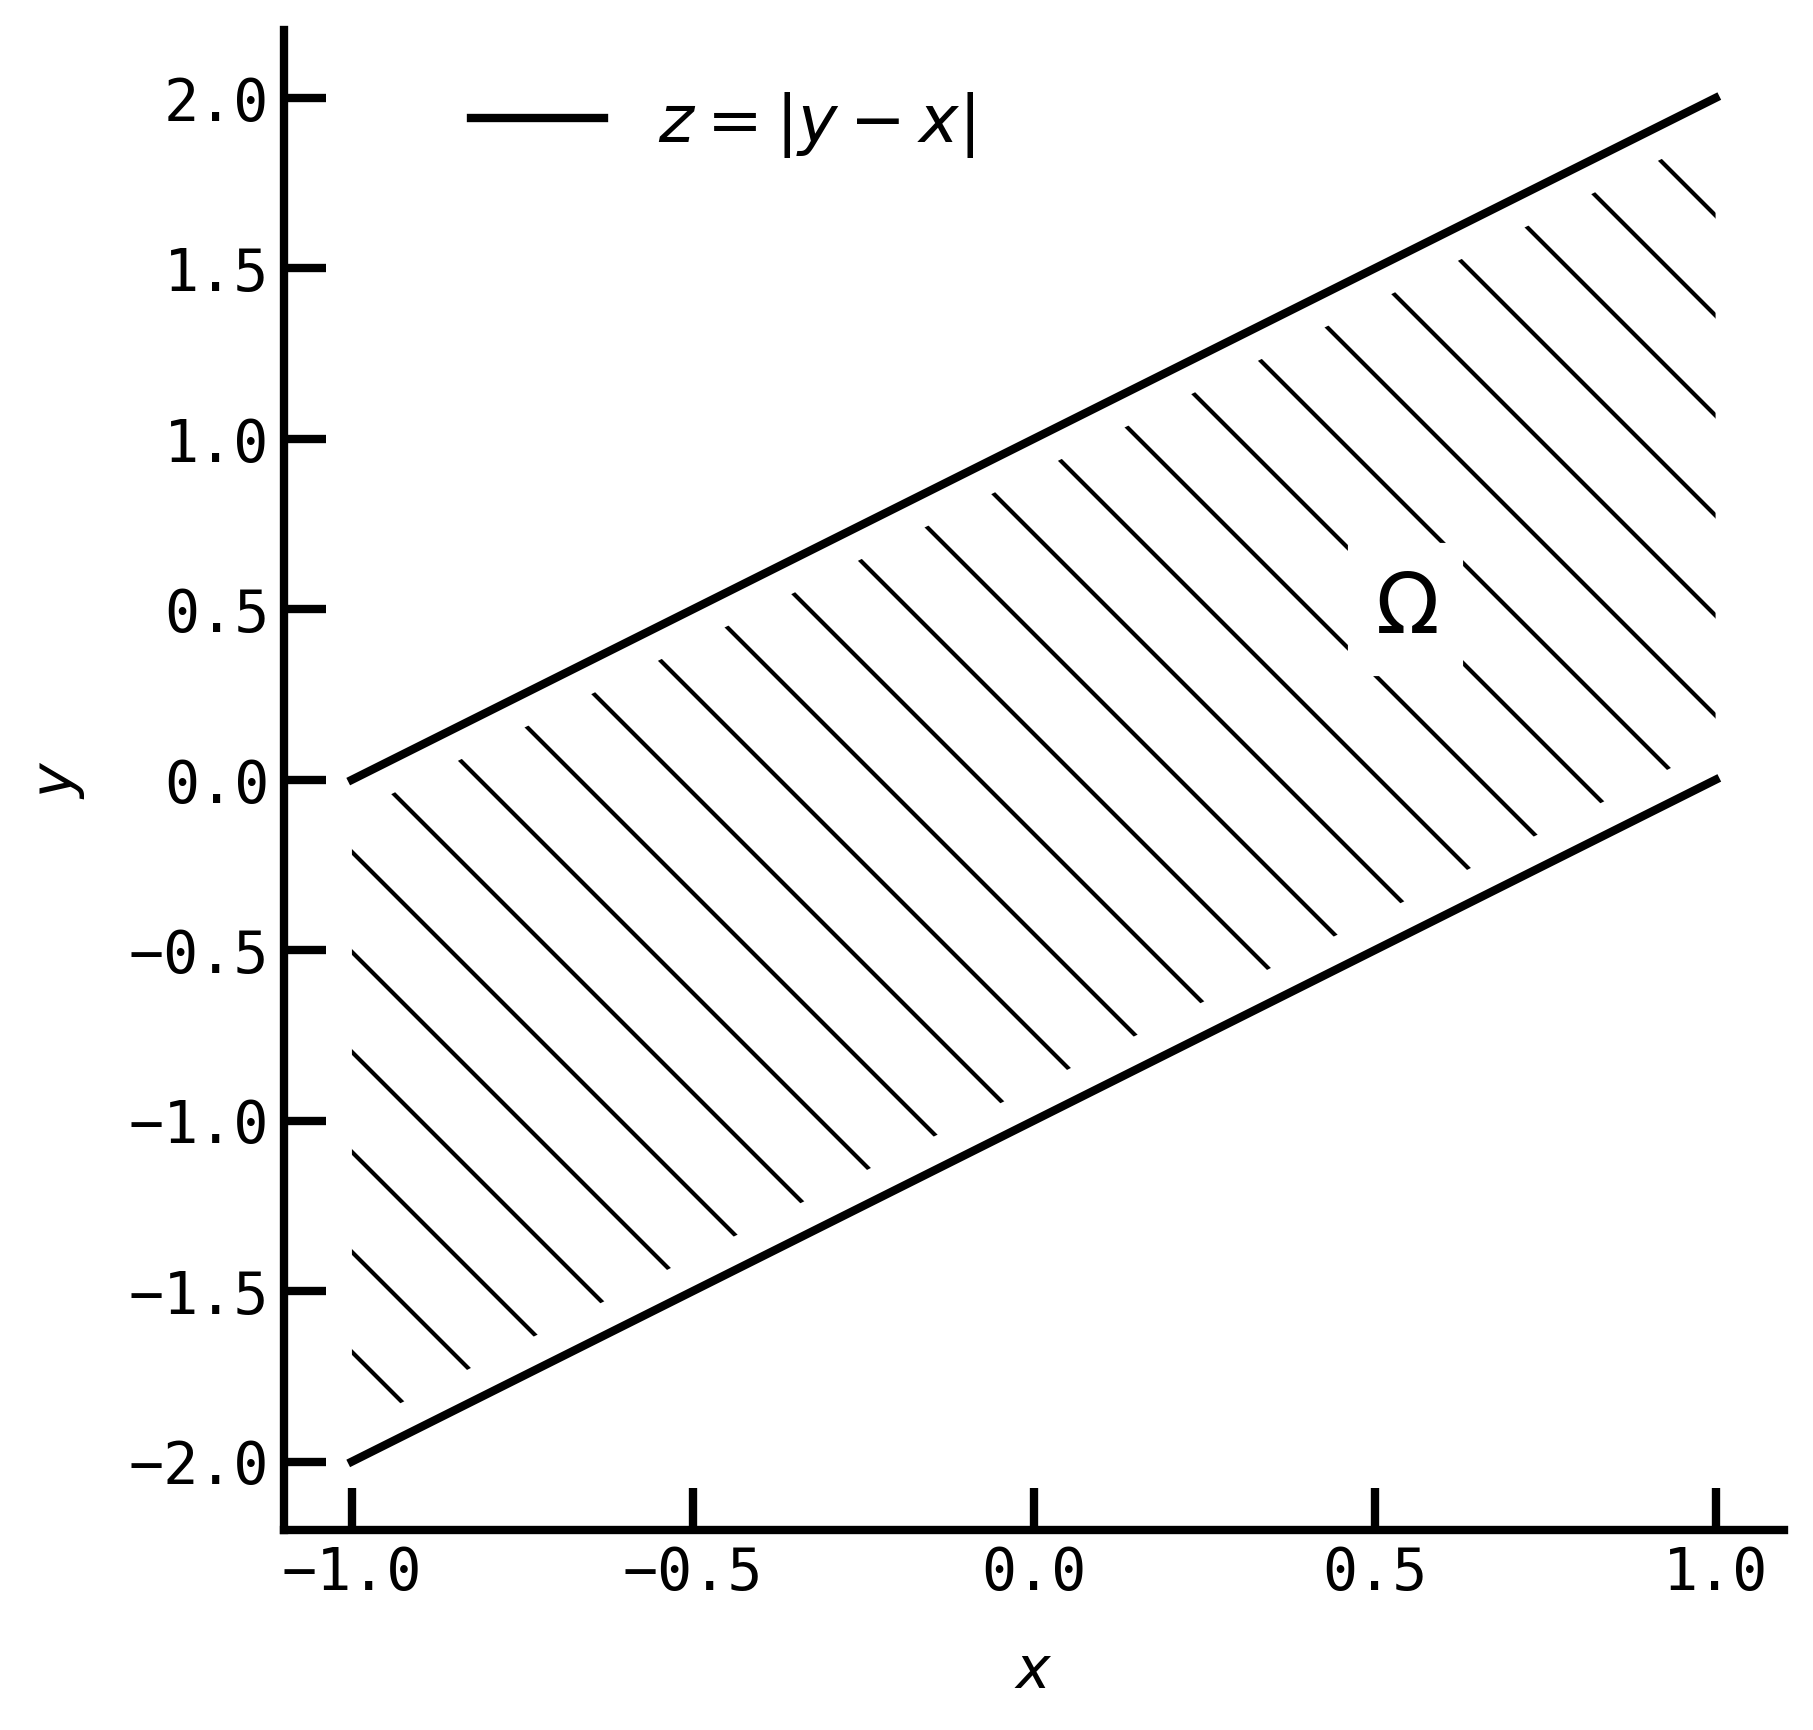
\includegraphics[width=0.5\linewidth]{img/abs_err_area}
	\caption{Joint density function domain $\Omega$}
	\label{fig:z-area}
\end{figure}


Let $F_Z(z)$ denote the distribution of the absolute difference in a single observation. The distribution function is given by:

\begin{equation}
	F(z) = \iint\limits_\Omega f_X(x) f_Y(y) \,dy\,dx = \int\limits_{-\infty}^{\infty} \int\limits_{x-z}^{x+z} f_X(x) f_Y(y) \,dy\,dx, ~ z \geq 0
	\label{eq:Fz}
\end{equation}

\begin{equation}
	f(z) = \frac{dF(z)}{dz} = \int\limits_{-\infty}^{\infty} f_X(x)\left( f_Y(x+z) + f_Y(x-z) \right)\,dx,~ z \geq 0
	\label{eq:fz}
\end{equation}

In the following sections, we examine important special cases of uncertainty distributions and their relationship to the absolute difference $|a-b|$ and the MAE $h$ from Equation~\ref{eq:gen_mae}.

\section{Data without uncertainty}

We first consider the idealized case of data without measurement uncertainty. In this scenario, the probability density functions for observations are characterized by Dirac delta functions:

\begin{equation}
	\begin{aligned}
		f_X(x) &= \delta(x-a) \\
		f_Y(y) &= \delta(y-b)
	\end{aligned}
	\label{eq:delta_ab}
\end{equation}

If $m = a - b$,
\begin{equation}
	\begin{aligned}
		f_X(x) &= \delta(x) \\
		f_Y(y) &= \delta(y-m)
	\end{aligned}
	\label{eq:delta_m}
\end{equation}

\begin{equation}
	f(z) = \delta(z-m) + \delta(z+m),~ z \geq 0, \forall m \in \mathbb{R} 
	\label{eq:fz_deltas}
\end{equation}

Characteristic function:
\begin{equation}
	\psi(t) = \int\limits_{0}^{\infty} e^{i\,t\,z}\,f(z)\,dz = e^{i\,|m|\,t}
	\label{eq:charf_deltas}
\end{equation}

Expected value and variance:
\begin{equation}
	\begin{aligned}
		E\left[Z\right] &= \frac{1}{i}\,\frac{d}{dt} \ln{\psi} \bigg|_{t=0} = \left\vert m \right\vert\\
		V\left[Z\right] &= -\frac{d^2}{dt^2} \ln{\psi} \bigg|_{t=0} = 0
		\label{eq:EV_delta}
	\end{aligned}
\end{equation}

Equation~\ref{eq:EV_delta} is consistent with the problem formulation: in the observation of random variables $X$ and $Y$, we can only obtain $x=a$ and $y=b$. Therefore, Equation~\ref{eq:fz_deltas} can be interpreted as the uncertainty distribution for data without measurement uncertainty, and the proposition in Equation~\ref{eq:delta_ab} is valid for this case.

The probability that the observed absolute difference $z$ is less than some value $z'$ is:
\begin{equation}
	P(z \leq z') = \int\limits_{0}^{z'} f(z)\,dz = \int\limits_{0}^{z'} \left[\delta(z-m) + \delta(z+m)\right]\,dz = H(z'-m) + H(z'+m) - 1,
\end{equation}

where $H(x)$ denotes the Heaviside step function.

From Equation~\ref{eq:P_delta}, it follows that the probability can only assume three distinct values:
\begin{equation}
	\begin{aligned}
		P(z \leq z') = 
		\begin{cases}
			0 & \text{if } |m| = 0,\, z' = 0 \text{ or } |m| > z'\\
			\frac{1}{2} & \text{if } |m| = z',\, z' > 0\\
			1 & \text{if } |m| < z'
		\end{cases}
	\end{aligned}
	\label{eq:P_delta}
\end{equation}

Since we have observed $z$, the probability $P(z \leq z')$ can only take values of $\frac{1}{2}$ or $1$ (indicated by the shaded area in Figure~\ref{fig:P_deltas}).

The case $P(z \leq z') = \frac{1}{2}$ represents a marginal uncertainty scenario because at $z' = |m| + \delta z$ we have $P(z \leq z') = 1$, while at $z' = |m| - \delta z$ we have $P(z \leq z') = 0$, where $\delta z$ is an infinitesimal variation of $z$.

\begin{figure}[H]
	\centering
	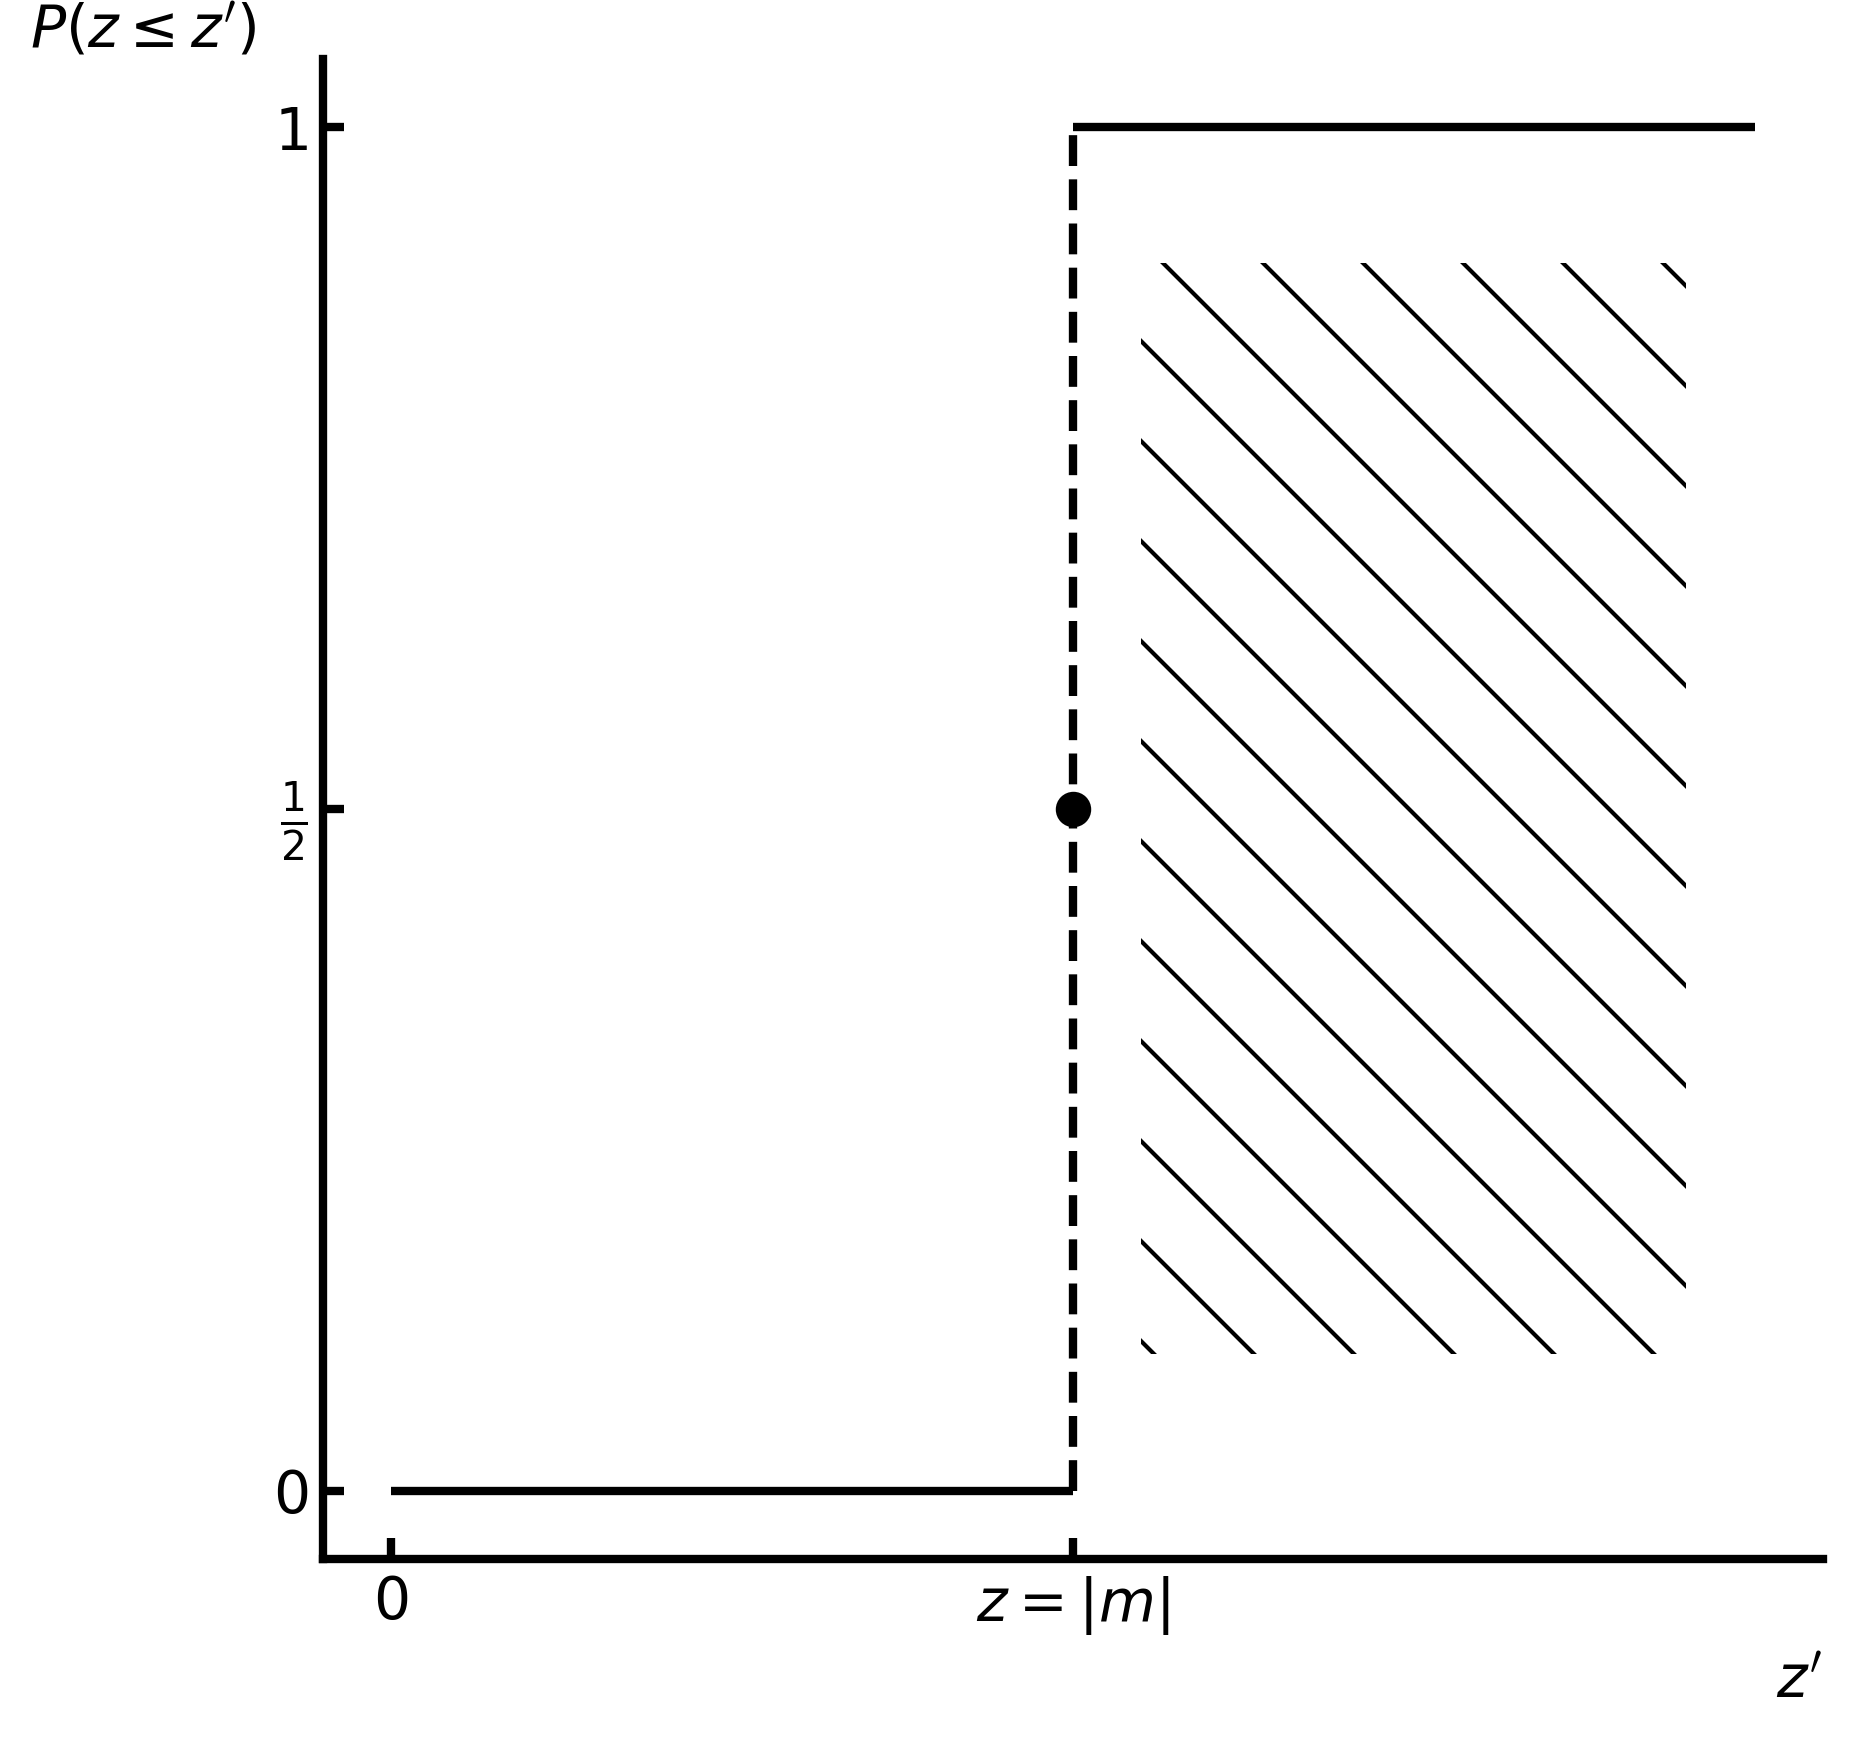
\includegraphics[width=0.5\linewidth]{img/P_deltas}
	\caption{Probability of $z \leq z'$. Patched area shows possible cases of $z'$ for observed value $z$.}
	\label{fig:P_deltas}
\end{figure}

Since $z=|m|$ (Equation~\ref{eq:EV_delta}), and defining $\varepsilon = z' - |m|$ as the tolerance for comparing $z$ and $|m|$ (equivalently, $|x-y|$ and $|a-b|$), the probability $P(z \leq z')$ represents the likelihood that the values $|x-y|$ and $|a-b|$ can be considered equivalent within tolerance $\varepsilon$.

For a series of observations $\{x_k\}$ and $\{y_k\}$, we examine the integral characteristic expressed by the random variable:
\begin{equation}
	W = \frac{1}{n} \sum\limits_{k=1}^{n} Z_k
	\label{eq:W}
\end{equation}

Using Equation~\ref{eq:EV_delta} and the properties of expected value and variance, we obtain:
\begin{equation}
	\begin{aligned}
		E\left[W\right] &= \frac{1}{n}\sum\limits_{k=1}^{n} E[Z_k] = \frac{1}{n}\sum\limits_{k=1}^{n} |m_k| = h\\
		V\left[W\right] &= \frac{1}{n^2}\sum\limits_{k=1}^{n} V[Z_k] = 0
		\label{eq:EV_Wdelta}
	\end{aligned}
\end{equation}

The condition required by Kolmogorov's strong law of large numbers, $\sum\limits_{k=1}^{\infty}\frac{V[Z_k]}{k^2} < \infty$, is clearly satisfied. Since $E\left[W\right]$ equals the MAE $h$ (Equation~\ref{eq:gen_mae}), we have:

\begin{equation}
	h = \frac{1}{n} \sum\limits_{k=1}^{n} z_k = \frac{1}{n} \sum\limits_{k=1}^{n} |x_k-y_k|, \text{ as } n\to\infty
	\label{eq:h_delta}
\end{equation}

Equation~\ref{eq:h_delta} represents the standard method for calculating MAE in practice. For the simple case of data without uncertainty (Equation~\ref{eq:fz_deltas}), this approach coincides with Equation~\ref{eq:gen_mae}. While the same result could be obtained directly from the fact that $a_k=x_k$ and $b_k=y_k$ for data without uncertainty, we have derived it using a general approach that relies only on the uncertainty distribution (Equation~\ref{eq:fz_deltas}) without explicit use of prior knowledge about the values of $a_k$ and $b_k$. This methodology can therefore be extended to more complex cases involving uncertainty described by other distributions.

It is important to note that Equation~\ref{eq:h_delta} is valid only for data without uncertainty; for other uncertainty distributions, the relationship will not have such a simple form.

However, in many practical applications involving dataset comparisons using absolute differences (e.g., MAE for model performance evaluation), MAE is calculated using the form of Equation~\ref{eq:h_delta} even when data contains uncertainty. This approach is generally incorrect and can lead researchers to erroneous conclusions. In the following sections, we explore the impact of uncertainty for two cases of significant practical importance.

\section{Data with normal distribution of uncertainty}

In this case, we assume that the individual estimations $x$ and $y$ follow normal distributions (Equation~\ref{eq:fxfy_norm}) with means $a$ and $b$, respectively. In practice, this scenario corresponds to most physical measurements obtained from sensors, measuring instruments, or mathematical/ML models where uncertainty in input data propagates to uncertainty in outputs. Thus, this case is applicable, for example, to the validation of such models against physical measurements in industrial projects (quality control, product property forecasting, etc.).

\begin{equation}
	\begin{aligned}
		f_X(x) &= \frac{1}{\sigma_x\sqrt{2\pi}}e^{-\frac{1}{2} \left(\frac{x-a}{\sigma_x}\right)^2}\\
		f_Y(y) &= \frac{1}{\sigma_y\sqrt{2\pi}}e^{-\frac{1}{2} \left(\frac{y-b}{\sigma_y}\right)^2}
	\end{aligned}
	\label{eq:fxfy_norm}
\end{equation}

Using Equation~\ref{eq:fz}, the uncertainty distribution $f(z)$ becomes:
\begin{equation}
	f(z) = \frac{1}{\sigma\sqrt{2\pi}}\,\left[e^{-\frac{1}{2} \left(\frac{m+z}{\sigma}\right)^2} + e^{-\frac{1}{2} \left(\frac{m-z}{\sigma}\right)^2}\right]
	\label{eq:fz_normal}
\end{equation}

where $m = a - b$ and $\sigma = \sqrt{\sigma_x^2 + \sigma_y^2}$.

By finding the characteristic function of the distribution in Equation~\ref{eq:fz_normal} and computing the corresponding derivatives, we calculate the expected value and variance for this distribution:
\begin{equation}
	\begin{aligned}
		E[Z] &= m\,\mathrm{erf}\left(\frac{m}{\sqrt{2}\,\sigma}\right)+\frac{\sqrt{2}\,\sigma\,e^{-\frac{1}{2}\left(\frac{m}{\sigma}\right)^2}}{\sqrt{\pi}}\\
		V[Z] &=  m^2+\sigma^2-E[Z]^2
	\end{aligned}
	\label{eq:EV_norm}
\end{equation}

As can be observed, Equation~\ref{eq:EV_norm} is symmetric with respect to the sign of $m$, so $m$ can be replaced by $|m|$. From the behavior of both components in the $E[Z]$ equation:
\begin{equation}
	E[Z] \geq |m|
	\label{eq:EZ_geq_m_norm}
\end{equation}

where equality $E[Z] = |m|$ is achieved only as $|m|\to\infty$. Note also from Equation~\ref{eq:EV_norm} that $V[Z]$ is a monotonically increasing function, so $\max\limits_{m\in\mathbb{R}} V[Z] = \lim\limits_{|m|\to \infty} V[Z] = \sigma^2$.

Summing over the entire series $\{z_k\}$:
\begin{equation}
	\frac{1}{n} \sum\limits_{k=1}^{n} E[Z_k] \geq \frac{1}{n}\sum\limits_{k=1}^{n} |m_k|
\end{equation}

In the series $\{z_k\}$, maximal value of Kolmogorov's condition achieved at $\forall |m_k|\to\infty$ will be:
\begin{equation}
	\begin{aligned}
		\lim\limits_{\forall|m_k|\to\infty} \sum\limits_{k=1}^{\infty}\frac{V[Z_k]}{k^2} &= \sum\limits_{k=1}^{\infty} \frac{\lim\limits_{|m_k|\to\infty} V[Z_k]}{k^2} = \sum\limits_{k=1}^{\infty} \frac{\sigma}{k^2} = \frac{\pi^2\,\sigma}{6} < \infty
	\end{aligned}
	\label{eq:kolm_norm}
\end{equation}

Easy to see, for any other $|m|$, sum from the left part of Eq.\ref{eq:kolm_norm} less than $\frac{\pi^2\,\sigma}{6}$. Thus, using Kolmogorov's theorem we have:
\begin{equation}
	\frac{1}{n} \sum\limits_{k=1}^{n} z_k \geq \frac{1}{n}\sum\limits_{k=1}^{n} |m_k| , \text{ as } n\to\infty
	\label{eq:means_zm}
\end{equation}

From Equation~\ref{eq:means_zm}, we observe that the mean of observed absolute differences is greater than the MAE and, in general, cannot be used as an MAE estimator, unlike the case of data without uncertainty considered previously. However, we can establish a sufficient condition for the approximation: 

\begin{equation}
	\frac{1}{n} \sum\limits_{k=1}^{n} z_k \approx \frac{1}{n}\sum\limits_{k=1}^{n} |m_k|
	\label{eq:mae_approx_norm}
\end{equation}

Due to the law of large numbers, Equation~\ref{eq:mae_approx_norm} can be written as:
\begin{equation}
	\frac{1}{n} \sum\limits_{k=1}^{n} E[Z_k] \approx \frac{1}{n}\sum\limits_{k=1}^{n} |m_k|
	\label{eq:mae_approx_norm_EZ}
\end{equation}

We make the following change of variables: 
\begin{equation}
	u_k = \frac{|m_k|}{\sqrt{2} \sigma}
	\label{eq:var_change}
\end{equation}

Therefore, the expression for $E[Z_k]$ (Equation~\ref{eq:EV_norm}) takes the form:
\begin{equation}
	E[Z_k] = \sqrt{2}\sigma \left[u_k \mathrm{erf}(u_k) + \frac{1}{\sqrt{\pi}}\,e^{-u_k^2}\right]
\end{equation}

Introducing a correction coefficient $\alpha \approx 1$, we can rewrite Equation~\ref{eq:mae_approx_norm_EZ} as:
\begin{equation}
	\sum\limits_{k=1}^{n} \left( u_k \mathrm{erf}(u_k) + \frac{1}{\sqrt{\pi}}\,e^{-u_k^2} \right) = \alpha \sum\limits_{k=1}^{n} u_k
	\label{eq:alpha}
\end{equation}

Differentiating Eq.\ref{eq:alpha} with respect to each $u_k$:
\begin{equation}
	\sum\limits_{k=1}^{n} \mathrm{erf}(u_k) = n\,\alpha
	\label{eq:alpha_diff}
\end{equation}

For convenience we can use the same correction coefficient for each part of the sum from Eq.\ref{eq:alpha_diff}. Thus,  
\begin{equation}
	\mathrm{erf}(u_k) = \alpha,\,\forall k
	\label{eq:alpha_095}
\end{equation}
is sufficient for Equation~\ref{eq:alpha_diff} to be satisfied. Therefore, if $u_k \geq \sqrt{2}$, then $\alpha \gtrsim 0.95$, which satisfies the condition $\alpha \approx 1$ in many cases.

Reverting the variable change (Equation~\ref{eq:var_change}), we obtain the sufficient condition for Equation~\ref{eq:mae_approx_norm}:
\begin{equation}
	|m_k| \gtrsim  2\sigma, \, \forall k
	\label{eq:mae_approx_condition}
\end{equation}

Therefore, Equation~\ref{eq:mae_approx_norm} can be applied only when the values in series $\{a_k\}$ and $\{b_k\}$ are sufficiently different (Equation~\ref{eq:mae_approx_condition}). Depending on the context and the degree of uncertainty expressed by $\sigma$, this condition may limit the applicability of Equation~\ref{eq:mae_approx_norm}. For example, in the context of model validation where $\{a_k\}$ represents model predictions compared against measurements $\{b_k\}$ under conditions of high data uncertainty (large $\sigma$), the applicability of Equation~\ref{eq:mae_approx_norm} will be limited to poorly performing models, which is insufficient for many applications.

Let us consider $E[Z]$ (Equation~\ref{eq:EV_norm}) as a function $\phi(m)$. Since $\phi(m)$ is a convex function, Jensen's inequality gives us:
\begin{equation}
	\phi(h) \leq \bar{\phi},
	\label{eq:ineq_jensen}
\end{equation}
where $\bar\phi$ is the mean of $\phi(m)$ over $\{m_k\}$: $\bar\phi = \frac{1}{n} \sum\limits_{k=1}^{n} z_k$ and $h = \frac{1}{n} \sum\limits_{k=1}^{n} m_k$, which corresponds to the MAE definition in Equation~\ref{eq:gen_mae}.

We define $\varepsilon$ as the relative difference between $\bar{\phi}$ and $\phi(h)$:
\begin{equation}
	\varepsilon = \frac{\bar{\phi} - \phi(h)}{\phi(h)}
\end{equation}

Using the maximum value of $\varepsilon$ and Equation~\ref{eq:ineq_jensen}, we obtain:
\begin{equation}
	\frac{1}{1+\varepsilon_{max}}\bar{\phi} \leq \phi(h) \leq \bar{\phi}
	\label{eq:phi_interval}
\end{equation}

Therefore, the accuracy with which we can determine $\phi(h)$ from Equation~\ref{eq:phi_interval}, and hence the MAE $h = \phi^{-1}(\phi(h))$, depends on $\varepsilon_{max}$, which we can estimate through numerical experiments.

Consider values from $\{m_k\}$ constrained to an interval $[\mu_1, \mu_2]$ and distributed uniformly. By varying the values of $\mu_2 \geq \mu_1 \geq 0$, we can calculate possible values of $\varepsilon$ and estimate its maximum value $\varepsilon_{max}$. The uniform distribution of $\forall m_k \in [\mu_1, \mu_2]$ is a good modeling choice for simulation because of its heavy tails; this provides a worst-case estimation of $\varepsilon$ compared to distributions with lighter tails, since greater dispersion over $[\mu_1, \mu_2]$ enhances the inequality in Equation~\ref{eq:ineq_jensen} over the interval.


\begin{figure}[H]
	\centering
	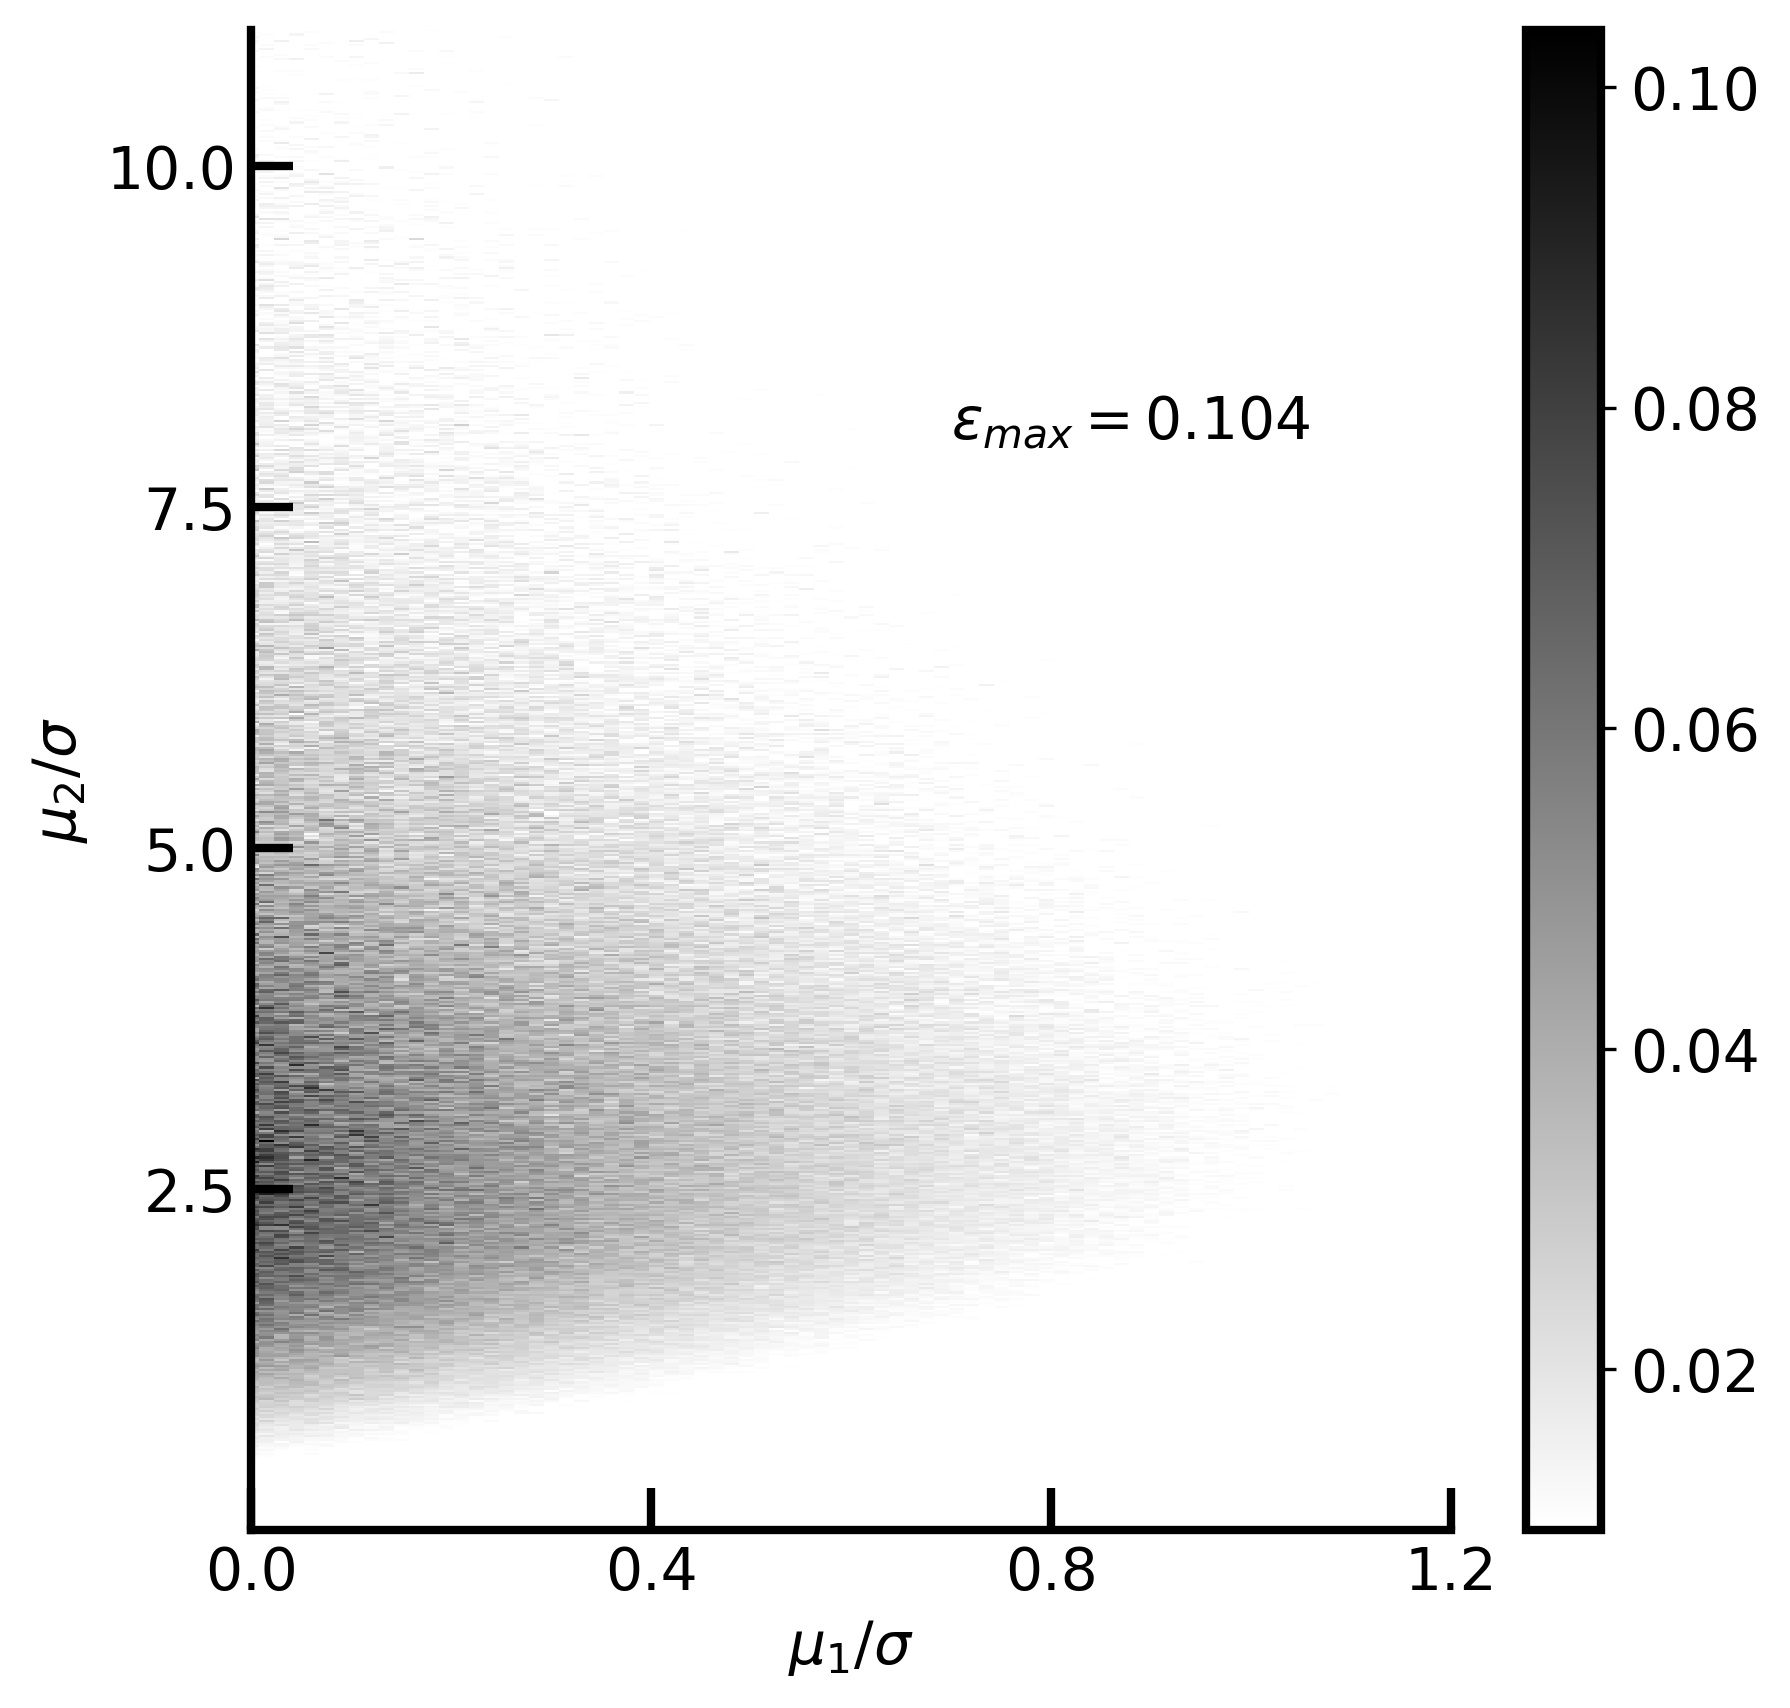
\includegraphics[width=0.5\linewidth]{img/eps_map}
	\caption{}
	\label{fig:eps_map}
\end{figure}

\begin{figure}[H]
	\centering
	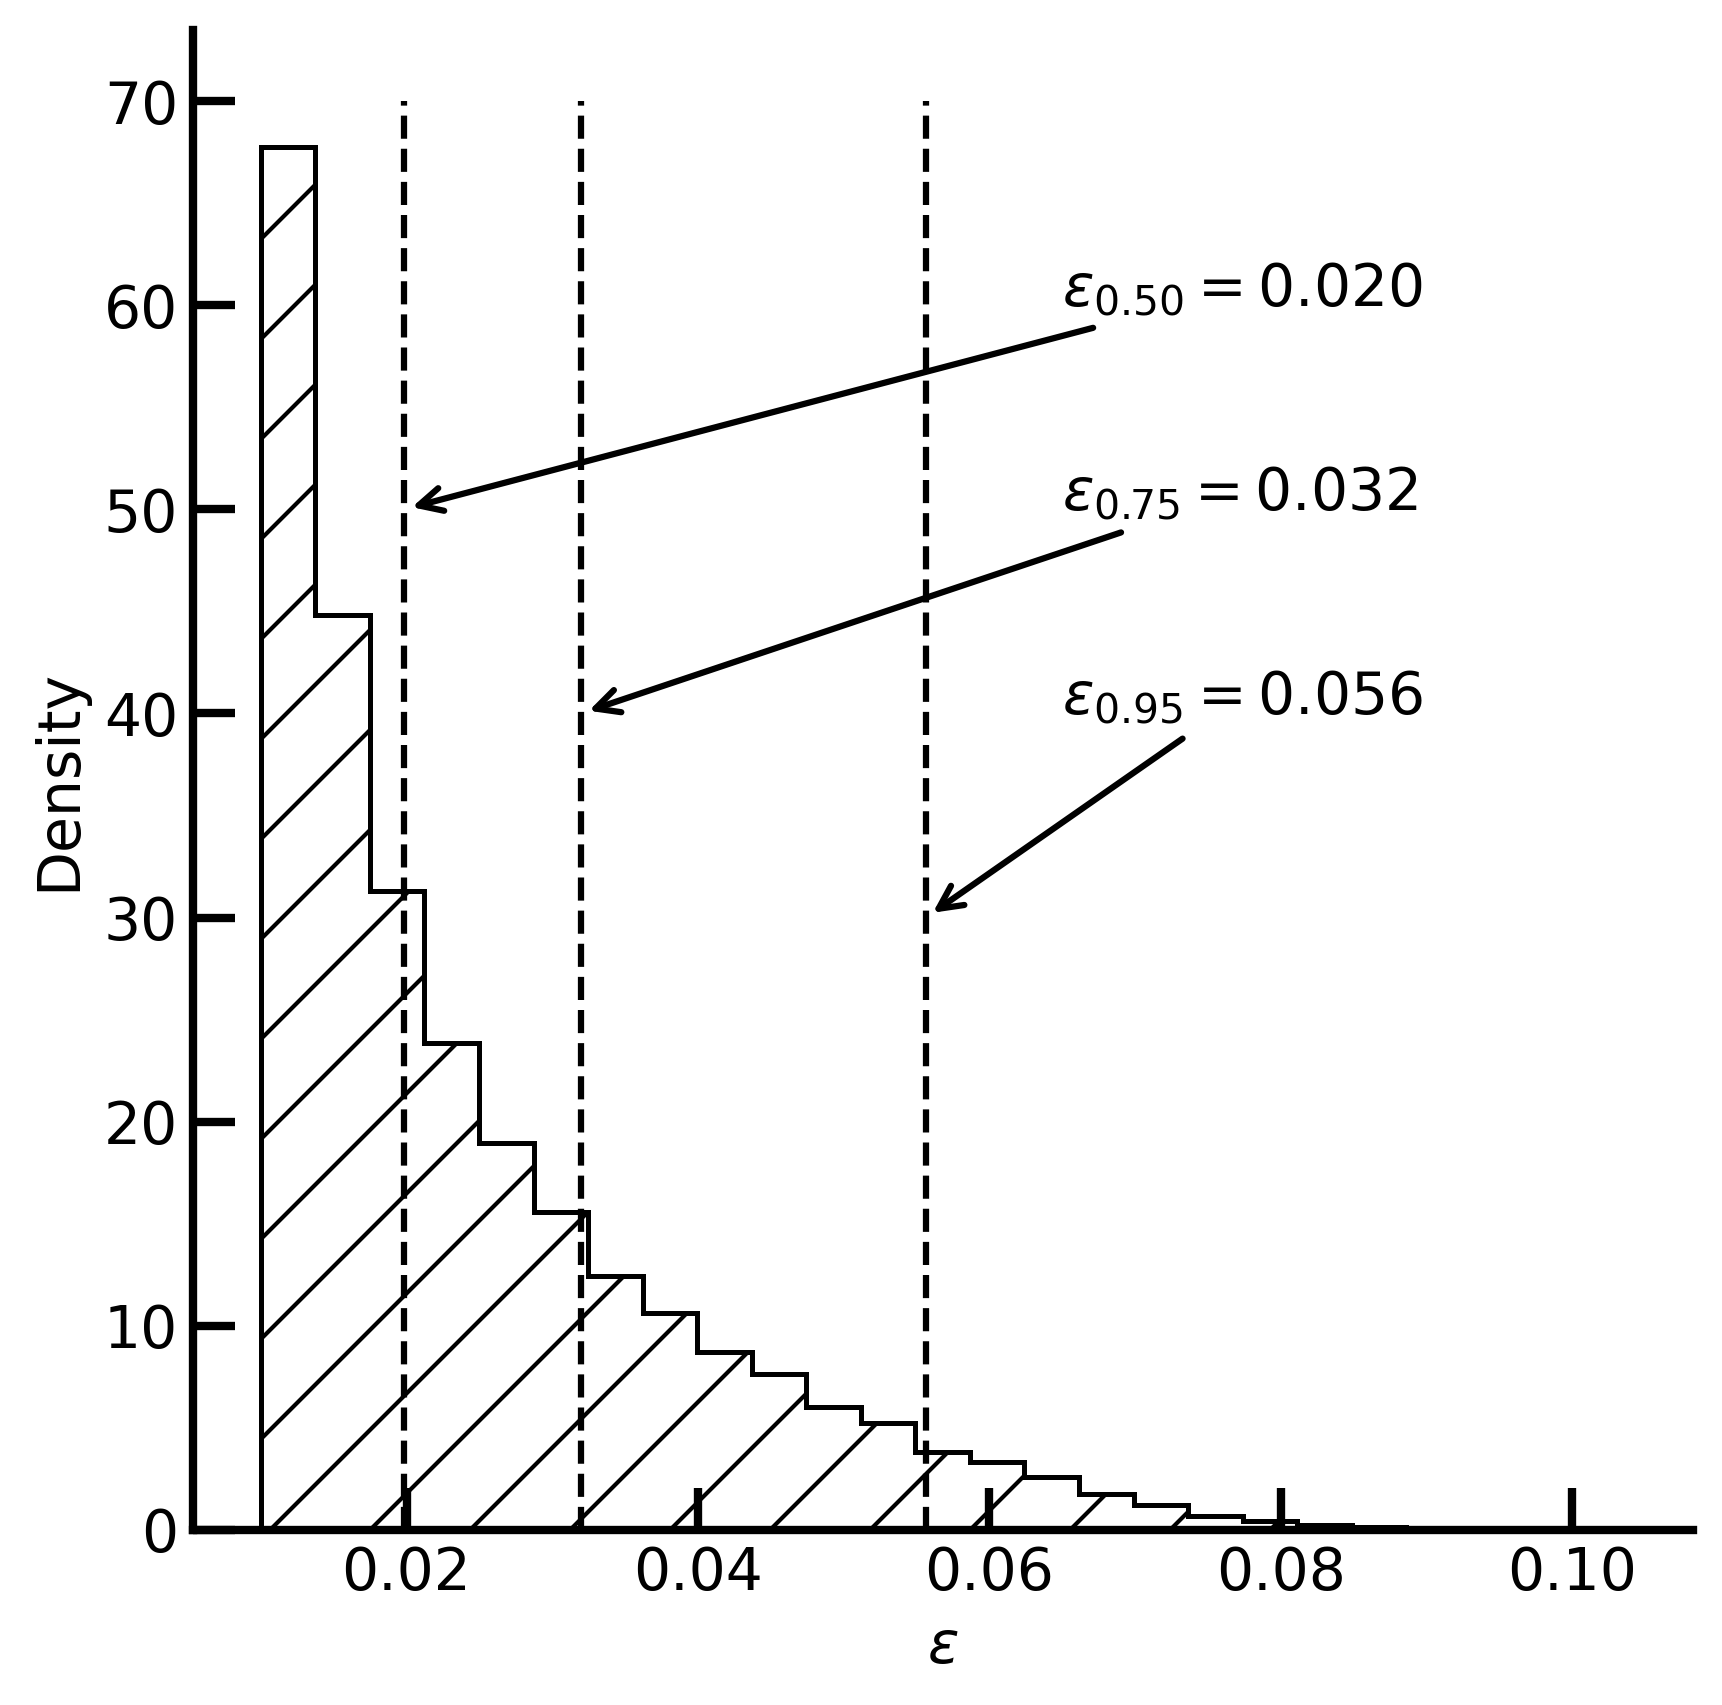
\includegraphics[width=0.5\linewidth]{img/eps_distr}
	\caption{}
	\label{fig:eps_distr}
\end{figure}

\begin{figure}[H]
	\centering
	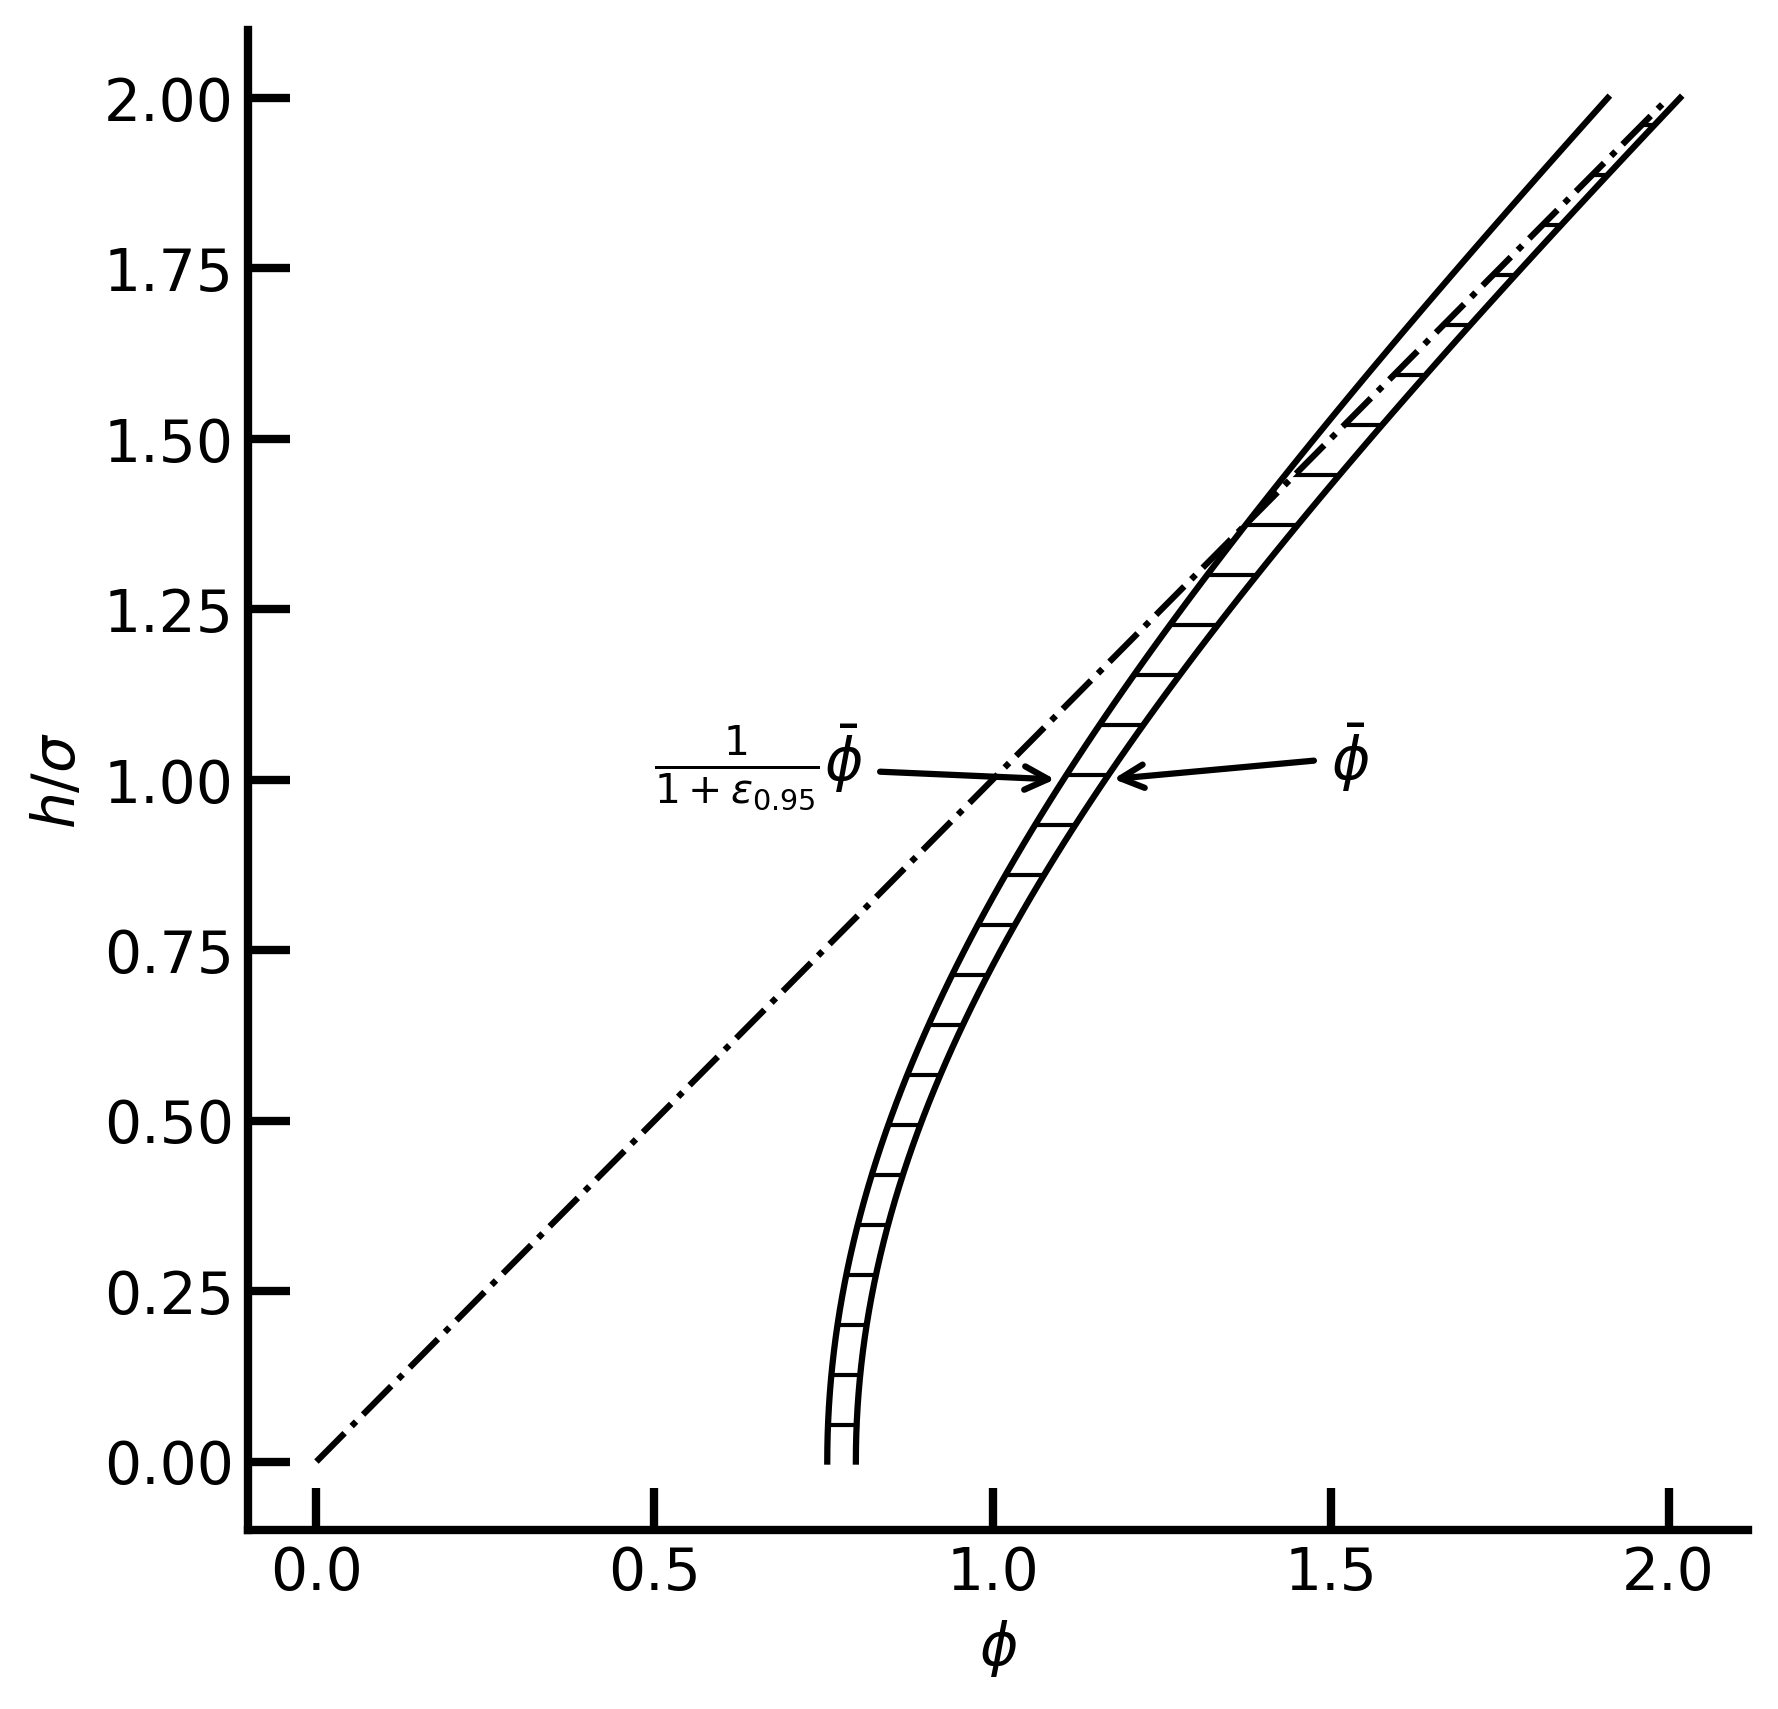
\includegraphics[width=0.5\linewidth]{img/h_phi}
	\caption{Accuracy of MAE $h$ determination}
	\label{fig:h_phi}
\end{figure}




\section{Mixed case: Market price dispersion example}

Consider the example of market price dispersion where different sellers have different offers for the same commodity. For instance, multiple real estate agents may want to sell the same house, each with their own selling strategy, resulting in prices distributed according to some probability distribution. In this scenario, prices are random variables.

Now imagine that a dataset contains prices from only one real estate agent. In this case, the true price, which should be determined by objective market circumstances, is unknown. Typically, predictive models are based on market indices rather than the psychology of a selected real estate agent, highlighting the importance of understanding measurement uncertainty in such applications.

\section{Conclusion}

\section{Acknowledgments}

\end{document}

